\documentclass[11pt]{article}

\usepackage[a4paper,margin=1.1in]{geometry}
\usepackage{amsmath,amssymb,amsthm,mathtools}
\usepackage{hyperref}
\usepackage{enumitem}
\usepackage[table]{xcolor}
\usepackage{mdframed}
\usepackage{array}
\usepackage{tikz}
\usetikzlibrary{arrows.meta,decorations.pathreplacing,calc}
\tikzset{
  var/.style={circle,draw,thick,fill=white,inner sep=1.5pt,minimum size=7mm,font=\small},
  win/.style={line width=9pt,line cap=round,draw=blue!12},
  up/.style={-{Stealth[length=2.2mm]},thick,blue!60!black},
}
\hypersetup{hidelinks}

\theoremstyle{plain}
\newtheorem{theorem}{Theorem}[section]
\newtheorem{lemma}[theorem]{Lemma}
\newtheorem{proposition}[theorem]{Proposition}
\theoremstyle{definition}
\newtheorem{definition}[theorem]{Definition}

\newcommand{\bbN}{\mathbb{N}}
\newcommand{\bbZ}{\mathbb{Z}}
\newcommand{\cD}{\mathcal{D}}
\newcommand{\cG}{\mathcal{G}}
\newcommand{\st}[1]{\textsf{\small[#1]}}
\newcommand{\precisely}[1]{\par\smallskip\noindent{\small\textit{Precisely:} #1}\par\smallskip}
\newcommand{\bp}[1]{\begin{mdframed}[backgroundcolor=black!4,linewidth=0.4pt]#1\end{mdframed}}

\title{Pointless Coherence on Glued Carriers}
\author{Patrick S.\ Mahon}
\date{October 2026}

\begin{document}
\maketitle

\bp{\large Answers can be consistent without being about anything, as long as
the contradiction hides in a question nobody can ask.}

\medskip
\noindent This note follows that sentence through two stories, a sandwich shop
and a county survey, and out the other side into a theory. The puzzles come first, because the theory is
only a careful account of what they show. Precise statements sit in short
\emph{Precisely} asides and in the appendix, where proofs and status labels
live (\st{Lean} machine-checked, \st{hand} my proof, \st{cited}
literature).

\tableofcontents

%======================================================================
\section{The sandwich shop}\label{sec:die}

A sandwich shop has six sandwiches on its menu. Each is made of exactly
\emph{two} of four fillings, so every pair of fillings appears once:
\begin{center}\small
\begin{tabular}{l | c c c c}
sandwich & cheese & ham & egg & tomato\\\hline
cheese \& ham & \checkmark & \checkmark & & \\
cheese \& egg & \checkmark & & \checkmark & \\
cheese \& tomato & \checkmark & & & \checkmark\\
ham \& egg & & \checkmark & \checkmark & \\
ham \& tomato & & \checkmark & & \checkmark\\
egg \& tomato & & & \checkmark & \checkmark\\
\end{tabular}
\end{center}
The online order form asks about one filling at a time: \emph{Cheese? yes/no.
Ham? yes/no. Egg? yes/no. Tomato? yes/no.} The owners wrote the form's
validation and know nothing about the menu. Their only rule: \textbf{every line
must be answered, with exactly one of yes or no.}

A picky customer submits \emph{no, no, no, no}. Does it pass validation?
\begin{center}\small
\begin{tabular}{l | c c | c}
line & yes & no & ticks\\\hline
Cheese? & & \checkmark & 1 \checkmark\\
Ham? & & \checkmark & 1 \checkmark\\
Egg? & & \checkmark & 1 \checkmark\\
Tomato? & & \checkmark & 1 \checkmark\\
\end{tabular}
\end{center}
Every line has exactly one tick, so the order is \emph{consistent}: it passes
the only check the owners know how to make.

Can the kitchen make it? Say a sandwich \emph{fits} the order if every answer on
the form is right for that sandwich. Hold each sandwich up against the order:
\begin{center}\small
\begin{tabular}{l | c c c c | l}
 & cheese? & ham? & egg? & tomato? & fits?\\\hline
\textbf{the order} & \textbf{no} & \textbf{no} & \textbf{no} & \textbf{no} & \\\hline
cheese \& ham & yes & yes & no & no & $\times$\\
cheese \& egg & yes & no & yes & no & $\times$\\
cheese \& tomato & yes & no & no & yes & $\times$\\
ham \& egg & no & yes & yes & no & $\times$\\
ham \& tomato & no & yes & no & yes & $\times$\\
egg \& tomato & no & no & yes & yes & $\times$\\
\end{tabular}
\end{center}
Every sandwich has two fillings, so nothing on the menu fits. A valid order the
kitchen cannot make.

Where did the contradiction go? Each line on its own was fine. Even ``no cheese,
no ham'' is fine, since egg \& tomato fits. The trouble appears only when all the
``no''s are combined, and the form has no line for combinations. ``No cheese
\emph{and} no ham \emph{and} no egg?'' is not a question on this form. The
contradiction lives in a question that is never asked.

This is the whole phenomenon in miniature. Here it is harmless: there are only
six sandwiches, nothing is infinite, and the cure is simply to add combination
lines to the form.\footnote{Mathematically this is an example of Navara and
Pt\'ak, \emph{\v{C}as.\ p\v{e}st.\ mat.}\ 108 (1983): six possibilities and four
yes/no questions, each possibility answering ``yes'' to exactly two.}

%======================================================================
\section{The survey offices}\label{sec:windows}

Now a county with infinitely many possibilities. Its villages each stand at some
height, a whole number of metres, and nobody has a map. The survey is run by
small offices, each covering \emph{two neighbouring villages}. An office answers
any question about its two villages, ``is this one higher than that one?'', ``is
the pair exactly $(30,70)$?'', and nothing else. As in the sandwich shop, new
questions can be built from these with ``not'' and with ``exactly one of these
options'', even infinitely many options, as in ``what is the height?''. A
\emph{head office} knows nothing about geography. It checks only that the
answers are \emph{consistent}: whenever a question is split into exclusive
options, the ``yes''es add up correctly, and two offices that share a village
say the same things about it.

Start with villages in a line, West to East, with offices covering
$\{x_0,x_1\}$, $\{x_1,x_2\}$, $\{x_2,x_3\}$. Here $x_k$ stands for the height
of village $k$. Every office reports: \emph{the village to the east stands
higher}.
\begin{center}
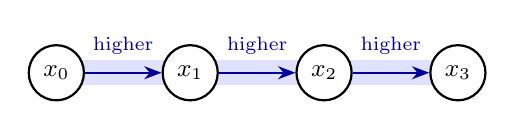
\begin{tikzpicture}[x=1.7cm]
\foreach \i in {0,1,2} \draw[win] (\i,0)--(\i+1,0);
\foreach \i in {0,...,3} \node[var] (n\i) at (\i,0) {$x_\i$};
\foreach \i/\j in {0/1,1/2,2/3} \draw[up] (n\i) -- node[above=3pt,font=\scriptsize]{higher} (n\j);
\end{tikzpicture}
\end{center}
\noindent The plain way to answer is from real heights, say $10,20,30,40$, reading
every answer off them. Those answers are fitted by an actual map.

There is a stranger way, which matters for everything that follows. An office
can describe a village as standing \emph{beyond every benchmark}. ``Is it 100
m?'' No. ``1{,}000 m?'' No. No to every particular height. ``Higher than any
figure you name?'' Yes. ``Is its height an even number?'' A definite yes or no,
fixed once and for all. That is a complete, consistent rule for answering every
question about one village. Call it an \emph{ideal height}.

\precisely{an ideal height is a non-principal ultrafilter $p$ on $\bbN$. Its
existence needs a little of the axiom of choice.}

An office can describe its \emph{pair} this way too, by imagining the two
heights \emph{drawn in turn} from the ideal rule, the eastern one \emph{later},
from even further out. ``Is the eastern village higher?'' Yes, since whatever
the western height is, almost every later draw beats it. Along a line this
always fits together. One ideal description of the whole county, ``draw $x_0$,
then $x_1$ later, then $x_2$, then $x_3$'', answers every question about all four
villages at once, and each office's answers are just its answers about two of
them. Call such a description of everything together an \emph{ideal map}. A real
map is an ideal map too, the trivial one.

\precisely{``draw $x_0$, then $x_1$ later'' is the ordered product $p\otimes p$:
a question $A$ about $(x_0,x_1)$ gets ``yes'' when $p$ says yes to the set of
$x_0$ for which $p$ says yes to $\{x_1:(x_0,x_1)\in A\}$. An ideal map is an
ultrafilter on the whole space of possibilities, an \emph{ideal point}; a real
map is a \emph{point}.}

On a line, then, consistent reports always come from some map, real or at worst
ideal. That turns out to be a theorem, not an accident (\S\ref{sec:why}).

%======================================================================
\section{Villages in a ring: the staircase}\label{sec:stair}

Now four villages in a ring, North, East, South and West, with offices covering
North--East, East--South, South--West and West--North. Every office reports:
\emph{the next village clockwise stands higher.}
\begin{center}
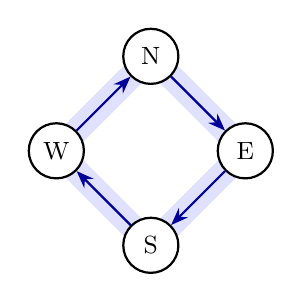
\begin{tikzpicture}
\foreach \k/\a/\n in {0/90/N,1/0/E,2/-90/S,3/180/W} \coordinate (r\k) at (\a:1.2);
\draw[win] (r0)--(r1); \draw[win] (r1)--(r2); \draw[win] (r2)--(r3); \draw[win] (r3)--(r0);
\foreach \k/\n in {0/N,1/E,2/S,3/W} \node[var] (q\k) at (r\k) {\n};
\draw[up] (q0)--(q1); \draw[up] (q1)--(q2); \draw[up] (q2)--(q3); \draw[up] (q3)--(q0);
\end{tikzpicture}
\end{center}
\noindent No real map can do this. Try a few against the reports:
\begin{center}\small
\begin{tabular}{l | c c c c | l}
heights (N, E, S, W) & E above N? & S above E? & W above S? & N above W? & fits?\\\hline
\textbf{the reports} & \textbf{yes} & \textbf{yes} & \textbf{yes} & \textbf{yes} & \\\hline
$10,20,30,40$ & yes & yes & yes & no & $\times$\\
$50,90,20,70$ & yes & no & yes & no & $\times$\\
$30,30,30,30$ & no & no & no & no & $\times$\\
\end{tabular}
\end{center}
Going round the ring, the heights must come back down somewhere, so every real
map gets at least one ``no''. It is a Penrose staircase, every step up and back
to the start.

Now let every office use ideal heights, each describing its pair as drawn in
turn, clockwise one later. Every office genuinely reports ``higher''. In the
West--North office it is North that is drawn later. Two offices that share a
village agree about it: both describe North by the same ideal rule, so ``is
North's height even?'' gets the same answer from either side.

Head office now checks \emph{everything}: every question that can be built from
the offices' answers, including combined questions spanning neighbouring
offices. Every check passes \st{Lean}. And the question that would expose the
staircase, ``is North lower than East lower than South?'', is not among them. No
office covers three villages, so it cannot be built from their answers, just as
the sandwich form had no line for combinations.
\begin{center}\small
\begin{tabular}{l | l | c}
check & what the reports say & passes?\\\hline
each office, alone & ``higher'': yes; ``exactly $n$ metres'': no for every $n$ & \checkmark\\
North, seen by West--North and North--East & the same answers (both by $p$) & \checkmark\\
every buildable question and its opposite & exactly one yes \st{Lean} & \checkmark\\
some real map fits & no: see the table above & $\times$\\
some ideal map fits & no: it would answer the forbidden question & $\times$\\
\end{tabular}
\end{center}

Why can there be no ideal map? An ideal map answers every question about all
four villages, the forbidden one included. It would have to say yes to North
below East below South below West below North.

So the reports are consistent and nothing fits them: no real map, and not even
an ideal one. Call such answers \textbf{pointless}. Each office's villages have
ideal heights; the county as a whole has no map at all. Each office has its own
sense of ``later'', and the ring closes those directions on themselves.

The sandwich order was pointless too, but trivially so, because the menu was
finite. The survey is pointless and infinite, and that is what makes it sharp.


%======================================================================
\section{What infinity demands}\label{sec:sigma}

Then the \emph{auditor} arrives. ``What is North's height?'' The auditor reads
out the list of every possible height, $0,1,2,\dots$, and asks for a yes beside
the right one. The offices say ``no'' to every height on the list, and ``yes'' to
``North has some height''.
\begin{center}
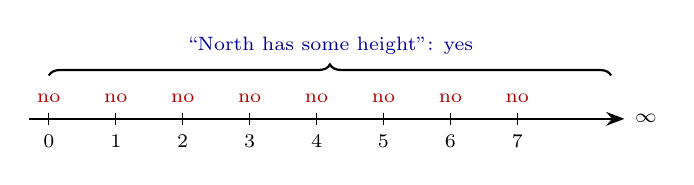
\begin{tikzpicture}[x=0.85cm]
\draw[thick,-{Stealth}] (-0.3,0)--(8.6,0) node[right,font=\scriptsize]{$\infty$};
\foreach \n in {0,...,7} {\draw (\n,0.08)--(\n,-0.08); \node[below,font=\scriptsize] at (\n,-0.08) {\n};
  \node[above,font=\scriptsize,red!70!black] at (\n,0.08) {no};}
\draw[decorate,decoration={brace,amplitude=4pt},thick] (0,0.55)--(8.4,0.55)
  node[midway,above=4pt,font=\scriptsize,blue!60!black]{``North has some height'': yes};
\end{tikzpicture}
\end{center}
\noindent Head office's rule only covers finite splits, and those are fine:
``at most 100 m?'' no, ``above 100 m?'' yes. The auditor's rule is stronger:
the ``yes''es must add up across \emph{infinitely} many options too. This is
$\sigma$-additivity, the usual rule of probability theory. Under it some single
height must get the yes. Every village is pinned to a real height, and real
heights cannot climb around a ring.

On these boards, demanding that answers add up over infinitely many options is
the same as demanding that they come from a real map
(Proposition~\ref{prop:sigma}). The auditor's demand for a completed answer is
exactly what makes the survey impossible.

%======================================================================
\section{Why loops: the first ideas of the theory}\label{sec:why}

The two stories show the whole mechanism. Separating its parts gives the
theory's first ideas.
From here on the story's words give way to general ones:

\begin{center}\small
\begin{tabular}{l l}
\textbf{story} & \textbf{general word}\\\hline
a village & a \emph{slot}\\
an office & a \emph{window}\\
an office's way of answering & a \emph{recipe}\\
a real map & a \emph{point}\\
an ideal map & an \emph{ideal point}\\
the offices and who covers what & the \emph{window graph}\\
\end{tabular}
\end{center}

\paragraph{Contradictions need questions that cannot be asked.} Consistent
answers respect every ``and'' that is actually on the board: if two questions
and their joint question can all be asked, two yeses force a yes on the joint
question (Lemma~\ref{lem:basic}). So a pattern can fail to be fitted only
through joint questions the board lacks. That is the space pointlessness lives
in.

\paragraph{No triangle keeps things local.} Questions put to windows that share
no slot always overlap, since they constrain different slots. So when a question
is split among several windows, those windows must pairwise share a slot. If the
window graph has no triangle, pairwise-touching windows always share one
\emph{common} slot: they form a star around it. Slicing at that slot shows that
the star's questions stay a star's questions under ``not''. The result is that
every buildable question is a question to one star of windows
(Theorem~\ref{thm:star}), so consistent answers are completely determined by what
each window says. This covers trees, every ring of length at least four, and
every other triangle-free graph. A triangle is the one shape where three windows
touch pairwise with no common slot, and there locality fails.
(In the language of hypergraphs: the windows have the \emph{Helly property}.)

\paragraph{Trees always glue.} Two neighbouring windows' ideal recipes, agreeing
on their shared slot, always combine into one recipe for all three slots
(Lemma~\ref{lem:amalg}). On a tree you can keep combining, one window at a time,
so on any tree, line or branching, every consistent pattern is an ideal point
(Theorem~\ref{thm:path}). Nothing pointless can happen without a loop.

\paragraph{Loops can carry a twist.} Around a loop the recipes may fail to
combine, as the staircase's directions do. Call a family of window recipes
\emph{flat} if it combines into one recipe for everything, and \emph{twisted}
otherwise. On triangle-free boards, a pattern is an ideal point exactly when its
window family is flat (Proposition~\ref{prop:flat}). Pointless patterns are
twisted families that still extend consistently to every buildable question.

\paragraph{Loops travel.} Suppose a board contains a loop of four or more windows
with no shortcut across it: no window joins two slots of the loop that are not
neighbours on it. Fix every slot off the loop at some number. As far as the
board's questions can tell, it is now the ring. A question to a window touching
the loop becomes a question about one loop slot, and a question off the loop
becomes trivially yes or no. So the staircase's answers carry over to the bigger
board, and they are still pointless there (Theorem~\ref{thm:travel}). Any board
with such a loop has pointless patterns, whatever else it contains.

\paragraph{Infinity forbids the twist.} Under $\sigma$-additivity every window is
pinned to actual numbers, and actual numbers carry no direction, so there is
nothing to twist.

\paragraph{The map so far.} Putting the boards together:
\begin{center}\small
\begin{tabular}{|>{\raggedright\arraybackslash}p{3.6cm}|>{\raggedright\arraybackslash}p{3cm}|>{\raggedright\arraybackslash}p{3.2cm}|>{\raggedright\arraybackslash}p{3.2cm}|}
\hline
& \textbf{tree} & \textbf{a shortcut-free loop of 4 or more} & \textbf{every loop has a shortcut} (triangles)\\
\hline
finitely many values & actual & actual & actual\\
\hline
infinitely many values, answers add up over infinitely many options & actual & actual & actual\\
\hline
infinitely many values, finite adding only & ideal \st{hand} & \cellcolor{orange!20}\textbf{pointless exists} \st{Lean ring + hand transport} & \cellcolor{yellow!25}\textbf{open}: the triangle decides\\
\hline
\end{tabular}
\end{center}
\noindent In graph language the columns are: forests; graphs with an induced cycle
of length $\ge4$ (non-chordal); and chordal graphs that are not forests. The
shaded cells are where the theory lives: a loop, infinitely many possibilities,
and only finite adding.

%======================================================================
\section{The open edge: the triangle}\label{sec:triangle}

Shrink the loop to three windows, $\{x_0,x_1\}$, $\{x_1,x_2\}$, $\{x_2,x_0\}$.
\begin{center}
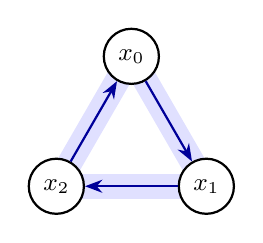
\begin{tikzpicture}
\foreach \k/\a in {0/90,1/-30,2/210} \coordinate (t\k) at (\a:1.1);
\draw[win] (t0)--(t1); \draw[win] (t1)--(t2); \draw[win] (t2)--(t0);
\foreach \k in {0,1,2} \node[var] (u\k) at (t\k) {$x_\k$};
\draw[up] (u0)--(u1); \draw[up] (u1)--(u2); \draw[up] (u2)--(u0);
\end{tikzpicture}
\end{center}
\noindent Now every two windows share a slot, but no slot is shared by all three:
the window graph is a triangle, the one shape the locality argument cannot
handle.
Questions can braid all three windows. With two possible values, ``are all three
equal?'' becomes askable, though it cannot be broken into window questions. With
three possible values that question disappears, and 2{,}088 others take its
place. The ring's method, reading every answer off neighbouring windows, no
longer applies.

So the triangle is the experiment that decides what the theory is about. Every
loop either has a shortcut-free stretch of four or more, which is already
settled, or is made of triangles.
\begin{itemize}[nosep]
  \item \emph{If the triangle carries pointless answers,} then so does every board
    with any loop. Triangles travel too, since a triangle never has a shortcut.
    Pointless coherence then happens \emph{exactly} on boards that are not
    trees.
  \item \emph{If it does not,} the expected line is \emph{chordal} versus
    \emph{non-chordal}: boards whose every long loop has a shortcut versus those
    with a shortcut-free one.
\end{itemize}
Either answer matches a classical pattern. Trees are where pairwise probability
tables always fit together (Wainwright--Jordan). Chordal graphs are where junction
trees and Vorob'ev's theorem live.
A computer check on a finite part of the board finds consistent answers. That
proves less than it seems. The finite part sees the slots only coarsely
(``bigger than 1?'', ``which is larger?''), so like the sandwich shop it can be pointless
for finite reasons alone. Whether the \emph{ideal}, infinite kind of
pointlessness happens on the triangle is genuinely open.

\paragraph{What the theory must settle.}
\begin{enumerate}[nosep]
  \item \emph{The invariant.} Not a tree, or not chordal? The triangle decides.
  \item \emph{Extension on triangle-free graphs.} There, a consistent pattern is
    the same as a family of window recipes that extends, and pointless means
    twisted (Theorem~\ref{thm:star}, Proposition~\ref{prop:flat}). Which twisted
    families extend? The rings say some do. Is it all of them, on every loop?
  \item \emph{The classification.} Which twisted families extend to every
    buildable question? The hope is that twist is measured by something like a
    winding number of the directions around each loop.
  \item \emph{Wider windows.} Windows showing three or more slots at once.
  \item \emph{No background at all.} The boards assume a space of
    \emph{possibilities} (the slots and their possible values) and nothing
    more. Drop even that, keeping only the questions. Does pointlessness
    survive when there is no space to lack a point in?
\end{enumerate}

%======================================================================
\section{Coda: where this sits}\label{sec:coda}

\paragraph{Its neighbours.} Each neighbouring theory covers a region and stops
at the edge of the shaded cells.
\begin{itemize}[nosep]
  \item \emph{Lines.} Vorob'ev (1962) and database theory show that consistent
    data on line-like structures always comes from a whole, for ordinary
    probabilities.
  \item \emph{Loops, with ordinary probabilities and finitely many outcomes.}
    The sheaf-theoretic account of contextuality owns this: Abramsky and
    Brandenburger, and for loops exactly, Kharoof, Ipek and Okay (2024).
  \item \emph{Infinity on ordinary (Boolean) boards.} De Finetti and Howson. On
    a board where every ``and'' can be asked, consistent answers are always ideal
    points.
\end{itemize}
None of them covers finitely additive answers on glued boards. That gap is
where this theory sits.

\paragraph{Its lineage.} The picture is old.
\begin{itemize}[nosep]
  \item \emph{Specker} opened the paper that became the Kochen--Specker theorem
    (1960) with a seer's three boxes. Any two opened hold exactly one gem, which
    is pairwise consistent and jointly impossible. That is the triangle.
  \item \emph{Penrose} explained the impossible staircase and tribar by the
    cohomology of a loop (1991).
  \item \emph{Aristotle} held that the infinite exists only potentially, never
    as a completed whole. Finite adding is the potential infinite. Adding up
    over infinitely many options is the actual one, and the staircase is a case
    where demanding the actual infinite excludes what the potential allows.
  \item \emph{Kant} called the completed series of conditions not \emph{given}
    but \emph{aufgegeben}, set as a task: ``nicht als Axiom, die Totalit\"at im
    Objekt als wirklich zu denken, sondern als ein Problem f\"ur den Verstand''.
    The staircase is a small antinomy. Every window is right, and the totality
    read as an object contradicts them, while read as a task it does not.
\end{itemize}

\paragraph{Its stance.} Throughout, answers come first. Nothing is assumed to
be giving them. Only the space of possibilities is assumed. Points, actual or
ideal, are what we get when answers can be reconstructed into a whole. The
theory is the study of when that reconstruction succeeds, and of what remains
when it fails.

%======================================================================
\appendix
\section{Definitions and results}\label{app:defs}

\begin{definition}[boards and answers]
A \emph{possibility space} is $\Omega=X^V$, with $V$ finite and $X$ an alphabet.
A \emph{window} is a two-element $\{i,j\}\subseteq V$, and the windows form a
graph. A \emph{window question} is $\{x:(x_i,x_j)\in A\}$ with $A\subseteq X^2$
arbitrary. The \emph{carrier} $\cD$ is the smallest family containing all window
questions and closed under complement and countable disjoint union: the
buildable questions. A \emph{state} (consistent answers) is
$s:\cD\to\{0,1\}$ with $s(\Omega)=1$ and $s(A\sqcup B)=s(A)+s(B)$ for disjoint
$A,B$. It is \emph{$\sigma$-additive} if additivity holds for countable disjoint
unions.
\end{definition}

\begin{definition}[points]
A state is a \emph{point} (fitted by an actual assignment) if
$s(E)=[\omega\in E]$ for some $\omega\in\Omega$. It is an \emph{ideal point} if
$s(E)=[E\in W]$ for an ultrafilter $W$ on $\Omega$. It is \emph{pointless} if it
is neither.
\end{definition}

\begin{lemma}\label{lem:basic}\st{hand; standard}
Let $s$ be a state on $\cD$.
\begin{enumerate}[label=(\alph*),nosep]
  \item If $A$, $B$ and $A\cap B$ are in $\cD$ and $s(A)=s(B)=1$, then
    $s(A\cap B)=1$.
  \item $s$ is an ideal point iff its true sets have the finite intersection
    property.
\end{enumerate}
\end{lemma}
\begin{proof}
\begin{enumerate}[label=(\alph*),nosep]
  \item $A\setminus B=(A\cap B^c)$ lies in $\cD$, being $A$ minus $A\cap B$, and
    lies inside $B^c$. So $s(A\setminus B)\le s(B^c)=0$.
  \item Extend the true sets to an ultrafilter; the false sets have true
    complements.
\end{enumerate}
\end{proof}

\begin{proposition}\label{prop:sigma}\st{Lean: ring, \texttt{no\_sigma\_extension};
hand: general}
If $X$ is countable, every $\sigma$-additive state on a glued carrier is a
point. If $X$ is finite, every state is a point.
\end{proposition}
\begin{proof}
\begin{itemize}[nosep]
  \item On each window the fibres $\{(x_i,x_j)=(a,b)\}$ form a countable (or
    finite) partition, so exactly one is true.
  \item Shared coordinates make these choices agree, giving one $\omega$.
  \item The sets on which $s$ agrees with $\delta_\omega$ form a carrier
    containing the window questions, hence all of $\cD$.
\end{itemize}
\end{proof}

\begin{theorem}[no triangle: locality]\label{thm:star}\label{lem:shape}\st{hand; machine-checked on finite alphabets}
Suppose the window graph has no triangle; equivalently, the windows form a Helly
family. Then every $E\in\cD$ is a disjoint union $\bigsqcup_i E_i$ of window
questions on windows that all contain one common coordinate (a star). So every
state satisfies $s(E)=\sum_i u_{w_i}(E_i)$ and is determined by its window
ultrafilters.
\end{theorem}
\begin{proof}
\begin{itemize}[nosep]
  \item \emph{Rigidity.} Window questions on windows with no shared coordinate
    meet if both are non-empty. So in a disjoint union of window questions, the
    non-empty pieces lie on pairwise adjacent windows. Without triangles, these
    form a star at some coordinate $c$.
  \item \emph{Slicing.} Fix $x_c=a$. Each piece's slice is a cylinder in its own
    leaf coordinate; they are pairwise disjoint in independent coordinates, so at
    most one is non-empty. The slice of $E^c$ is then a cylinder in the same
    coordinate, or everything. Gathering slices by leaf writes $E^c$ as a star at
    $c$.
  \item \emph{Closure.} Let $\cG$ be the disjoint unions of one window question
    per window. It is closed under complement (by slicing) and under countable
    disjoint union (regroup window by window). So $\cG=\cD$.
\end{itemize}
Machine check of $\cD=\cG$ (\texttt{notes/open\_questions/verification/glued\_helly\_check.py}):
\begin{itemize}[nosep]
  \item holds on the star $K_{1,3}$ (binary and ternary), a branching tree, the
    4- and 5-cycles, and $K_{2,3}$;
  \item fails whenever there is a triangle: triangle $70$ vs $66$; triangle with
    pendant $98$ vs $94$; 4-cycle with chord $148$ vs $132$.
\end{itemize}
Compare Greechie's loop lemma (Kalmbach 1983, \S4 L9).
\end{proof}

\begin{lemma}[gluing]\label{lem:amalg}\st{hand; very likely folklore}
Ultrafilters on $X\times Y$ and $Y\times Z$ with the same $Y$-marginal are the
projections of one ultrafilter on $X\times Y\times Z$.
\end{lemma}
\begin{proof}
Members of the two ultrafilters project into the common marginal, so they meet;
the sets $A\times Z$ and $X\times B$ have the finite intersection property.
\end{proof}

\begin{theorem}[trees]\label{thm:path}\st{hand}
If the window graph is a forest, every state is an ideal point.
\end{theorem}
\begin{proof}
\begin{itemize}[nosep]
  \item Order each tree's windows so that each meets the earlier ones in one
    coordinate.
  \item Glue the window ultrafilters one at a time (Lemma~\ref{lem:amalg}). Join
    separate trees by the product of their ultrafilters.
  \item This gives $W$ projecting to every $u_w$.
  \item By Theorem~\ref{thm:star}, $s(E)=\sum_iu_{w_i}(E_i)=\sum_iW(E_i)=W(E)$.
\end{itemize}
\end{proof}

\begin{theorem}[loops travel]\label{thm:travel}\st{hand, from the Lean ring witness}
If the window graph contains an induced cycle of length $L\ge4$, there is a
pointless state over $\bbN$ with no $\sigma$-additive version. If the triangle
carries a pointless state, so does every graph containing a triangle.
\end{theorem}
\begin{proof}
\begin{itemize}[nosep]
  \item Let $C$ be the induced cycle. Define $\psi:\bbN^C\to\bbN^V$ by copying the
    cycle coordinates and setting every other coordinate to a constant.
  \item Pull back each window question of the graph:
    \begin{itemize}[nosep]
      \item a window on the cycle gives a window question of the ring, since
        the cycle is induced, so there is no chord;
      \item a window from the cycle to outside gives a question about one ring
        coordinate;
      \item a window off the cycle gives $\emptyset$ or everything.
    \end{itemize}
  \item The sets whose preimage is in $\cD_C$ form a carrier, so
    $\psi^{-1}(\cD_G)\subseteq\cD_C$. Hence $s=\mu\circ\psi^{-1}$ is a state, with
    $\mu$ the ring witness (Theorem~\ref{thm:witness}).
  \item \emph{Pointless.} An ultrafilter fitting $s$ would push forward, along
    the projection to the cycle coordinates, to one fitting the staircase on the
    ring.
  \item \emph{No $\sigma$-additive version:} Proposition~\ref{prop:sigma}.
  \item \emph{The triangle clause:} the same argument, since a triangle is
    always induced.
\end{itemize}
The Lean development already proves the analogous transport along cycle maps
(\texttt{pullback}, \texttt{sL\_sigmaEssential}); this graph form is not yet in
Lean.
\end{proof}

\begin{proposition}[flatness]\label{prop:flat}\st{hand}
On a triangle-free window graph, a state is an ideal point iff its
window ultrafilters glue to one ultrafilter on $\Omega$ (a flat family).
\end{proposition}

\begin{theorem}[the staircase]\label{thm:witness}\st{Lean: \texttt{mu\_cases},
\texttt{sL\_sigmaEssential}}
For every $L\ge4$, the window ultrafilters $u_k=p\otimes p$ on the ring extend to
a state on the whole carrier over $\bbN^L$. No ultrafilter on $\bbN^L$ projects
to all $u_k$, since every $\{x_k<x_{k+1}\}$ would be in it, and their
intersection is empty. So the state is pointless, and by
Proposition~\ref{prop:sigma} it has no $\sigma$-additive version.
\end{theorem}
\noindent At $L=4$ the carrier's centre is literally $\{\emptyset,\Omega\}$ and
all six admissibility conjuncts hold (Lean, \texttt{D4\_six\_conjuncts}). No
prior-art owner was found in three passes.

\section{Status, sources, files}\label{app:status}

\paragraph{Status.}
\begin{itemize}[nosep]
  \item \st{Lean}: Theorem~\ref{thm:witness}; Proposition~\ref{prop:sigma} on the
    ring.
  \item \st{hand}: everything else in Appendix~\ref{app:defs}.
  \item Open: \S\ref{sec:triangle}.
  \item Prior-art risk for the staircase: Bhaskara Rao, \emph{Theory of
    Charges}; Goldberg on ultrafilter products.
\end{itemize}

\paragraph{Sources for the coda}, with how each was checked:
\begin{itemize}[nosep]
  \item read in full:
    \begin{itemize}[nosep]
      \item Kant, \emph{KrV}, Antinomy \S\S7--8 (German, Gutenberg ed.);
      \item Specker, \emph{Dialectica} 14 (1960), in Seevinck's translation,
        arXiv:1103.4537;
      \item Kharoof--Ipek--Okay, arXiv:2406.19961;
    \end{itemize}
  \item confirmed through bibliographic records only: Penrose, \emph{Structural
    Topology} 17 (1991);
  \item confirmed through secondary sources only: Aristotle, \emph{Physics}
    III.6; Vorob'ev 1962; Howson 2008.
\end{itemize}

\paragraph{Files.}
\begin{itemize}[nosep]
  \item Index: \texttt{glued\_carriers\_taxonomy.json}.
  \item Witness and prior art:
    \texttt{notes/open\_questions/delay\_embedding/collision\_vs\_generation.md}.
  \item Lean: \texttt{formalization/staging/WindowGluing.lean}.
  \item Relation to the cycle side:
    \texttt{cyclic\_marginal\_scoping.md}.
\end{itemize}

\end{document}
